\documentclass{article}

\usepackage{float,algorithm,graphicx,amsmath,amsfonts,verbatim}
\usepackage[noend]{algpseudocode}
\usepackage[hyphens]{url}

\title{Lab 10 - Unsupervised Learning}
\author{Kyle Swanson}
\date{January 29, 2018}

\setcounter{section}{-1}

\begin{document}

\maketitle

\section{Introduction}

In today's lab we are going to tackle some of the challenges of unsupervised learning, which is the task of learning features directly from unlabelled data. This is a much harder task as the lack of labels limits what we are able to learn, but there are still a number of interesting and useful applications of unsupervised learning. In particular, we will be learning about three unsupervised learning techniques: dimensionality reduction, clustering, and autoencoders.

\section{Dimesionality Reduction}

Dimensionality reduction is the process of simplifying our data representation by decreasing the dimensionality of the feature vectors representing each data point. Ideally we want to decrease the dimensionality of the data without losing too much of the information that distinguishes each data point from the others. To do this, we will implement the principal components analysis (PCA) method for performing dimensionality reduction, and we'll compare it to other dimensionality reduction methods. Dimensionality reduction is very useful for visualizing data (as we'll see in this lab), and it can also be used as a preprocessing step for other machine learning methods since learning from low dimensional data is easier and faster and it becomes harder to overfit.

In this part of the lab, we will be working with a set of 8x8 pixel grayscale images of hand-written digits. Go into \texttt{main.py} and uncomment Part 1 (only up to Part 1.1) and run \texttt{python main.py}. You'll see an image containing a selection of the digit images that we'll be working with (also displayed below).

\noindent
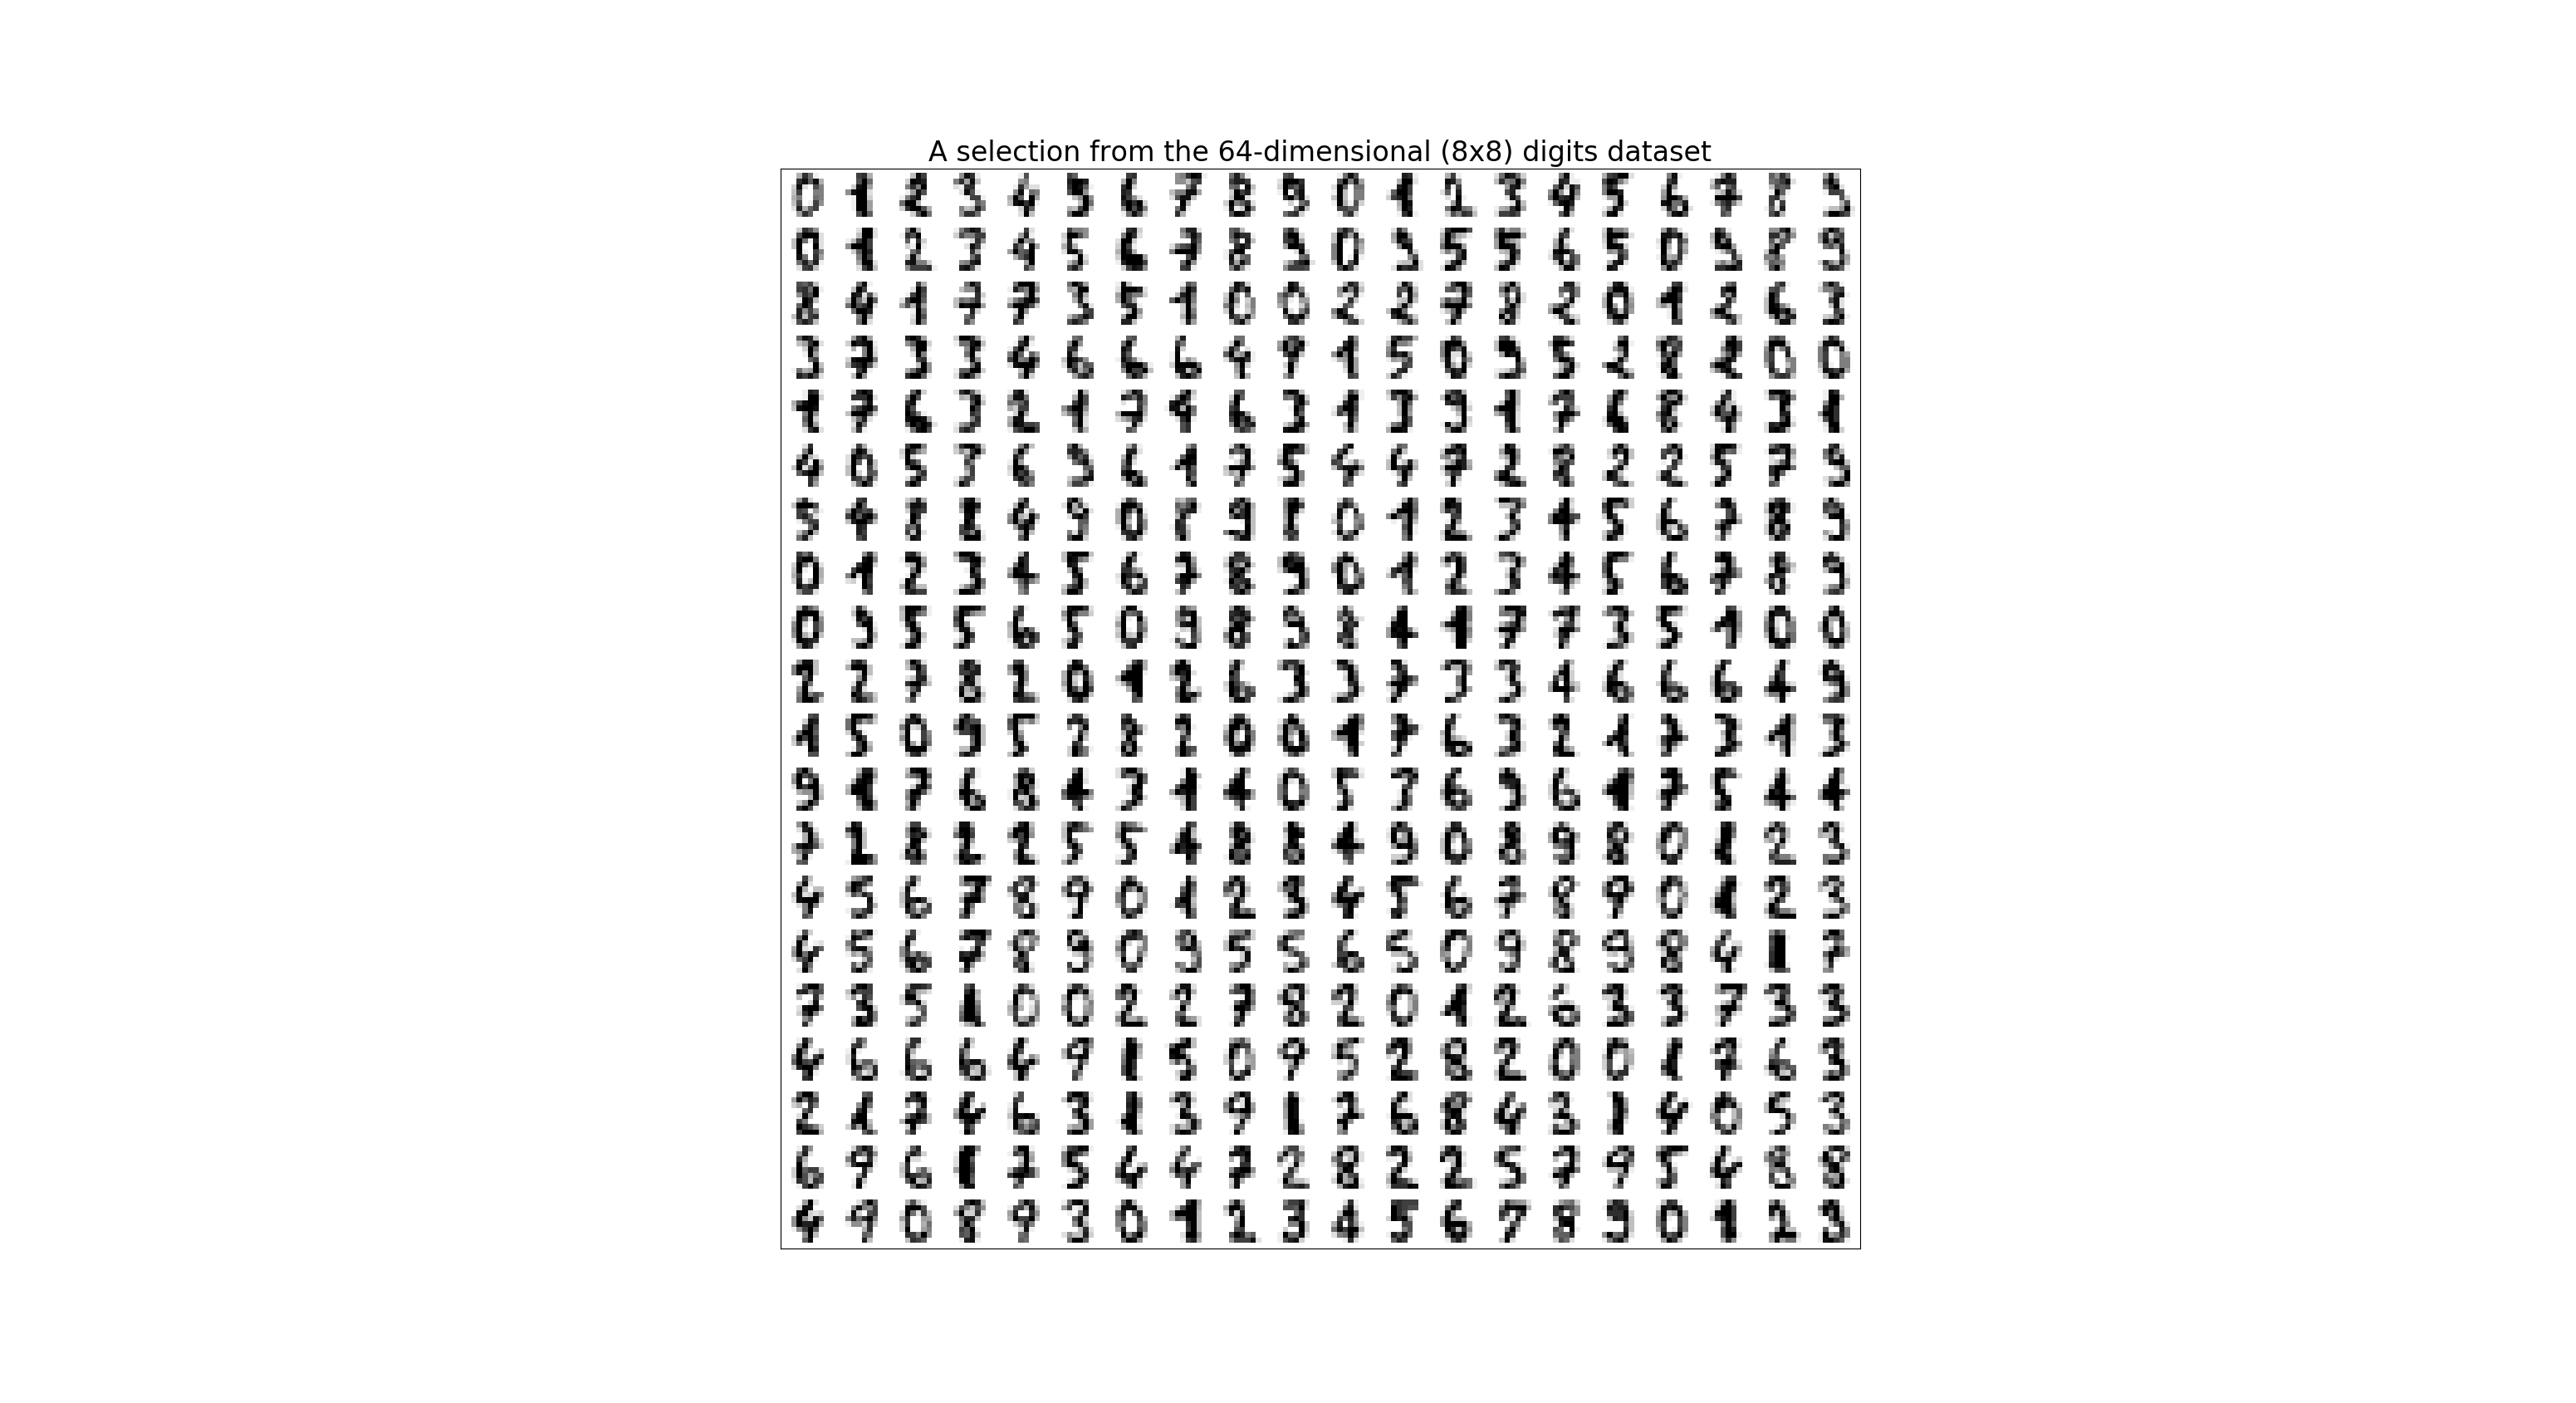
\includegraphics[width=\textwidth]{digits.png}

Since the images are 8x8 pixels, they are 64-dimensional. Visualizing a point in 64-dimensional space is impossible, so our goal will be to reduce the 64-dimensional vector to a 2-dimensional vector that we can plot. However, we still want our 2-dimensional reduction to contain the characteristics of the original 64-dimensional image; specifically, images of the same digit (ex. two different images of a 3) should end up nearby in 2-dimensions since the original 64-dimensional images were similar, while images of different digits (ex. an image of a 3 and an image of a 4) should end up far away in 2-dimensions since the original 64-dimensional images were different.

We'll see that randomly projecting a 64-dimensional vector to 2-dimensions will lose the characteristics of the original images, while using PCA or a more advanced method called t-SNE will result in 2-dimensional vectors which capture at least some of the characteristics of the original images.

\subsection{Random Projection}

First, we'll try to reduce our 64-dimensional images to 2 dimensions randomly. We will do this by generating a random 2 by 64 matrix and multiplying it by our 64-dimensional vector, which will result in a 2 dimensional vector. In Part 1.1 in \texttt{main.py}, I've done this random projection to 2 dimensions using sklearn's \texttt{SparseRandomProjection} model. Uncomment this code and run \texttt{main.py}. You'll see an image displaying the digits after being reduced to 2 dimensions. You can see that when the reduction is done randomly, the digits are all mixed together and we've lost all information separating the digits from each other. This is clearly a very bad method for dimensionality reduction.

\subsection{Principal Components Analysis (PCA)}

Principal components analysis (PCA) is a very common method for dimensionality reduction since it is (relatively) simple and is quick to compute. PCA works by computing the combinations of features (the principal components) which explain the greatest variance in the data (i.e. the greatest difference between data points). This can be done using some knowledge of linear algebra. We'll first write a PCA solver from scratch, then we'll use sklearn's implementation.

(For more information on PCA, you can find a great tutorial here: \url{https://towardsdatascience.com/a-one-stop-shop-for-principal-component-analysis-5582fb7e0a9c} and a cool demo here: \url{http://setosa.io/ev/principal-component-analysis/})

\subsubsection{PCA from scratch}

First we will implement PCA from scratch. Go into \texttt{lab10.py} and find the \texttt{PCA} class. Your job is to implement the \texttt{fit} and \texttt{transform} methods.

The \texttt{fit} method needs to learn the transformation matrix which will transform our data matrix with original features into a data matrix with principal components (different combinations of features) as features. We can do this with the following steps:

\begin{enumerate}
    \item Center and standardize the input data $X$. This means that for each column, you need to subtract the mean value of that column and divide by the standard deviation of that column. After performing this transformation, each column should have a mean of 0 and a standard deviation of 1. Call the centered and standardized matrix $Z$.
    
    (Note: Since some columns may have a standard deviation of 0 and dividing by 0 will result in an error, you should divide by the standard deviation plus some very small constant, such as \texttt{1e-6}.)
    
    \item Compute the covariance matrix of $Z$. The covariance matrix is $Z^T Z$ (this is matrix multiplication, so use \texttt{np.dot}). Call the covariance matrix $C$.
    
    \item Compute the eigendecomposition of $C$. This can be done with \texttt{np.linalg.eig(C)}. This will return a tuple with two values: the first is a numpy vector with eigenvalues (conveniently sorted in descending order) and the second is a numpy matrix where each column is an eigenvector. Set \texttt{self.Q} equal to the eigenvector matrix; this is going to be the matrix we use to transform our data into its principal components form in the \texttt{predict} method.
    
    \item We also want to know how much each principal component explains the variance in the data. The size of the eigenvalue indicates the amount that each eigenvector (principal component) explains variance. Set \texttt{self.explained\_variance\_ratio\_} equal to the vector of eigenvalues divided by the sum of the eigenvalues. This will give us a vector with the percent that each principal component explains the variance. We'll use this vector later to plot the amount of variance explained.
    
    \item \texttt{return self}
\end{enumerate}

Now we need to implement the \texttt{transform} method, which will use our transformation matrix \texttt{self.Q} to transform our data into its principal components. This can be done as follows:

\begin{enumerate}
    \item Center and standardize the data matrix $X$ the same way as you did in the fit method. Again, call this matrix $Z$.
    
    \item Transform $Z$ into its principal components by computing $ZQ$, where $Q$ is \texttt{self.Q} which you computed in the \texttt{fit} method (again, this is matrix multiplication, so use \texttt{np.dot}). Call this matrix $Z_{pc}$.
    
    \item Select only the most important principle components and throw out the rest. The number of components that we're going to keep is \texttt{self.n\_components}. To do this, select all the rows (i.e. all the data points) but only the first \texttt{self.n\_components} columns (principal components) of $Z_{pc}$ and save it as a new matrix called $Z_{pc\_reduced}$. Return this matrix.
    
    Note: This is where the dimensionality reduction actually happens. Up until this point, we simply transformed the data from one set of 64-dimensional features (the original features) to another set of 64-dimensional features (the principal components). But here we only select the top few principal components to keep as features of the data, so we have reduced the dimensionality of the data to the number of principal components that we keep.
\end{enumerate}

When your implementation is complete, uncomment Part 1.2.1 in \texttt{main.py} and run the file. First you'll see two plots illustrating the amount of variation explained by each principal component. On the left you'll see the proportion explained by each component, and on the right you'll see a graph of the cumulative variance explained. If you look at the cumulative graph, you should see that using just 2 principal components instead of all 64, we can still explain about 30\% of the variance in the data, meaning our 2-dimensional reduction will still contain a decent amount of the characteristics of the original 64-dimensional data. After closing this plot, you'll see a plot of the reduced data itself. You should see that, unlike with the random projection, the digits are somewhat clustered together, meaning PCA does a good job of maintaining the defining characteristics of the digits despite reducing the dimensionality by a factor of 32.

\subsubsection{PCA from sklearn}

Just for comparison, try uncommenting and running Part 1.2.2 in \texttt{main.py}, which uses sklearn's implementation of PCA. Even though the results may look different, you should see that the quality of the reduction is roughly similar (both separate the digits to a similar degree).

\subsection{t-SNE}

While PCA works well in many cases, there is a more advanced method of dimensionality reduction called t-distributed stochastic neighbor embedding (t-SNE, pronounced "tee-snee"), which can produce far superior results, though it runs much slower than PCA. Uncomment Part 1.3 in \texttt{main.py} and run the file. After waiting for 20-30 seconds, you should see a plot of the dimensionality reduction performed by t-SNE. You should see that it nearly perfectly separates the digits.

(For more on t-SNE and to see some cool visualizations, take a look at this article: \url{https://distill.pub/2016/misread-tsne/})

\section{Clustering}

Clustering involves identifying groups within a set of data points. The most common method for clustering, which we'll implement in this section, is the k-means algorithm, which learns how to group data points into $k$ clusters. Clustering has a range of applications, two of which we'll explore here. After implementing and testing the k-means algorithm, we'll use k-means to identify topics among a selection of news articles, and then we'll use k-means to perform image compression by clustering colors.

\subsection{K-Means Algorithm}

The k-means algorithm is an effective method for identifying clusters in data. It works by first guessing the centers of clusters, and then alternately assigning points to clusters and then recomputing the cluster centers according to the points assigned to each cluster. We will first implement the k-means algorithm from scratch, and then we will compare our model with with the k-means model from sklearn. Both will be tested on the t-SNE reduction of the 8x8 digits dataset from Part 1.3.

Uncomment Part 2.1 (up to Part 2.1.1) in \texttt{main.py}.

\subsubsection{K-Means from scratch}

Go into \texttt{lab10.py} and find the \texttt{KMeans} class. Your job is to implement the \texttt{fit} and \texttt{predict} methods.

The goal of the \texttt{fit} method is to learn the centers of the $k$ clusters. The algorithm works as follows:

\begin{enumerate}
    \item Initialize variables to keep track of the best (minimum) cost and the best set of cluster centers.

    \item Repeat \texttt{self.n\_iter} times:
    
    \begin{enumerate}
        \item Initialize the cluster centers to be randomly selected data points. (While the k-means algorithm I described in class initializes the centers to totally random values, I found that initializing them to random data points worked better.)
    
        \item Repeat while the cost changes:
        
        \begin{enumerate}
            \item Compute the assignments of points to clusters. This means you should compute an array with the number of the cluster that each data point belongs to. Data points are assigned to the cluster whose center is closest to that data point. (Hint: the sklearn function \texttt{pairwise\_distances\_argmin} is useful here.)
            
            \item Compute the cost of the cluster centers. The cost is the sum of the distances from each cluster center to all the points assigned to that cluster.
            
            \item Compute the new cluster centers. The center of each cluster is the mean (average) of all the data points in the cluster.
        \end{enumerate}
        
        \item If the cost is less than the best cost, set the best cost equal to the cost and set the best cluster centers equal to the cluster centers.
    \end{enumerate}
    
    \item Set \texttt{self.cluster\_centers\_} equal to the best cluster centers.
    
    \item \texttt{return self}
\end{enumerate}

The \texttt{predict} method works as follows: For each data point, predict the cluster whose center is closest to that data point. Return an array with the predictions.

Once your implementation is complete, go into \texttt{main.py}, uncomment Part 2.1.1, and run the file. After waiting a few seconds for t-SNE and k-means to run, you should see the plot of the t-SNE reduced digits with colored regions indicating the k-means clusters. White X's indicate the cluster centers. You should see that the colored regions predicted by k-means closely match the clusters that appear in the data.

\subsubsection{K-Means from sklearn}

For comparison, uncomment Part 2.1.2 in \texttt{main.py} and run the file. This will run sklearn's implementation of the k-means algorithm on the t-SNE reduced digits. You should see results which look very similar to yours.

\subsection{Clustering text documents with K-Means}

Next we will use k-means to cluster text documents which fall into one of four categories: baseball, automobiles, Windows, space.

Uncomment Part 2.2. You don't have to write any code, but observe what's happening. We're first loading a dataset of news articles pertaining to one of the above four categories. Then we're performing a feature extraction called latent semantic analysis (LSA), which is similar to PCA. LSA converts the text documents into low-dimensional feature vectors. Next, we perform k-means to cluster the documents based on these features. Finally, we extract the top 10 features from each cluster, and determine the word associated with each feature. Try running \texttt{main.py}. You'll see these words printed to the screen.

You can see that even though k-means was never told what the categories were or which documents belonged to which category, it was still able to discover clusters just based on the features (words) which best distinguished the news articles from each other.

\subsection{Image compression with K-Means}

Another cool application of k-means clustering is image compression. A standard image is a matrix of pixels, each of which contains 3 numbers: one for the amount of red, one for the amount of green, and one for the amount of blue (RGB). Each pixel can take on any of 256 values, making for a maximum of 16,777,216 colors. In this part, we're going to take a picture which contains 96,615 unique colors (see below), and we're going to use k-means to reduce the number of colors to 64. k-means will do this by finding clusters of similar colors, all of which will be replaced with the color of the center of the cluster. We'll then compare this to randomly selecting 64 colors and converting each of the 96,615 colors to the closest of those random 64 colors.

\noindent
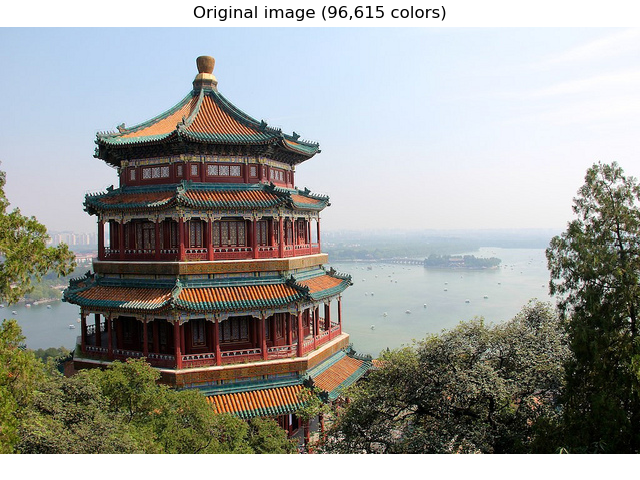
\includegraphics[width=\textwidth]{china.png}

Uncomment part 2.3 and run \texttt{main.py}. You'll see the original image with 96,615 colors, the image with the k-means selected 64 colors, and the image with the randomly selected 64 colors. Note how the image with the 64 colors selected by k-means looks very similar to the original image despite using about 1,500 times fewer colors, while the randomly selected 64 colors looks significantly different. This demonstrates that k-means can effectively compress the colors of an image to save space without the image losing much of its quality.

\section{Autoencoders}

Autoencoders are a method of performing unsupervised learning with neural networks. The network consists of two components: an encoder and a decoder. The encoder takes the original input and transforms it into an encoded representation, which is typically much smaller than the original input (the autoencoder compresses the input). The decoder then takes the encoded representation and attempts to transform it back to match the original input. The reconstruction created by the decoder is compared to the original input, and the autoencoder is optimized to minimize the difference between its reconstruction and the original input. Below is an illustration.

\noindent
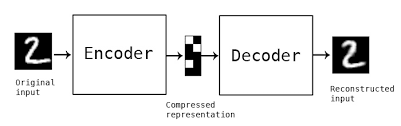
\includegraphics[width=\textwidth]{autoencoder.png}

Uncomment Part 3 (up to Part 3.1) in \texttt{main.py}.

\subsection{Image reconstruction with autoencoders}

First we will build an autoencoder and demonstrate its ability to reconstruct images. While autoencoders can take on a variety of architectures, we will be building the simplest version: a single layer fully connected neural network for the encoder and for the decoder. The encoder will use a relu activation, while the decoder will use a sigmoid activation to map the outputs to values between 0 and 1 (which can then be converted to pixel values).

Go into \texttt{lab10.py}. Your job is to implement the \texttt{build\_autoencoder} function. This function should return a keras Model with the following layers:

\begin{itemize}
    \item Input, shape=(\texttt{original\_dim},)
    
    \item Dense, \texttt{encoding\_dim} neurons, relu activation
    
    \item Dense, \texttt{original\_dim} neurons, sigmoid activation
\end{itemize}

When your implementation is complete, go into \texttt{main.py} and uncomment Part 3.1.

Before running the file, we're going to load a cool visualization tool called Tensorboard, which is provided by Tensorflow, the neural network package that keras uses in the backend. You can see in \texttt{main.py} that we're using \texttt{Tensorboard} when we're fitting the model in Part 3.1. To see the Tensorboard visualization, open a new terminal and type \texttt{tensorboard --log\_dir=/tmp/autoencoder}. Then open a web browser and navigate to \texttt{127.0.0.1:6006}. You'll see the Tensorboard visualization tool.

Now, in your first terminal window, run \texttt{python main.py}. While the model trains, look at the Tensorboard visualization. Click on the ``Graphs" tab to see a visualization of the autoencoder architecture. Click on the ``Scalars" tab to see a real-time visualization of the loss of the model. You should see the loss go down as the model trains.

(If you like the visualization, you can use Tensorboard in Parts 3.2 and 3.3 as well, though you should use \texttt{tensorboard --log\_dir=/tmp/denoising} for Part 3.2 and \texttt{tensorboard --log\_dir=/tmp/vae} for Part 3.3.)

After training is complete, you'll see an image with two rows of digits. The top row shows the original images while the bottom row shows the reconstructions of the autoencoder. Even though the autoencoder compressed the original 784-dimensional image (28x28 pixels) into a 32-dimensional vector (the \texttt{encoding\_dim}), which is a compression factor of 24.5, the autoencoder was still able to build a good reconstruction of the image.

\subsection{Image denoising with autoencoders}

Next we will use your autoencoder for a cool application: image denoising. Uncomment Part 3.2. In this part, the input to the autoencoder is a noisy image and output of the autoencoder is compared against a clean version of the image, thus training the autoencoder to remove noise from images. Run \texttt{main.py}. After training, you'll see an image with two rows of images. On the top are the original, noisy images, and on the bottom are the denoised images produced by the autoencoder. Despite the high volume of noise, the denoised images produced by the autoencoder are impressively clean.

\subsection{Image generation with variational autoencoders}

Finally, we will use a variant of an autoencoder called a variational autoencoder to generate new images of digits. Rather than doing a simple compression, a variational autoencoder tries to learn the underlying probability distribution of the digits. Then, by sampling from this probability distribution and running the samples through the decoder (now called a generator), it tries to reconstruct the input image.

While the learning process is the same as that for a regular autoencoder (it tries to minimize the difference between its reconstruction and the original input), the fact that it learns the underlying probability distribution means that we can sample from this probability distribution to generate new images (this is our first generative model!). Different samples will produce digits with different characteristics. Since variational autoencoders are more complicated than regular autoencoders, I've provided an implementation for you in \texttt{lab10.py} (based on \url{https://blog.keras.io/building-autoencoders-in-keras.html}).

Uncomment Part 3.3 in \texttt{main.py} and run the code. After training is complete, you'll first see two rows of digits, with the top row showing the original images and the bottom row showing the reconstructed images. While the quality may be a little worse than that of the regular autoencoder, the variational autoencoder uses an encoding dimension of 2 (here called \texttt{latent\_dim}), so the compression factor is much larger.

After closing this image, you'll see another image which displays the 2-dimensional encodings of the input images. So our variational autoencoder is actually performing dimensionality reduction from 784-dimensions to 2-dimensions (in Part 1 we were only reducing from 64-dimensions to 2-dimensions). While the digits aren't perfectly separated, the results are still impressive for using only 0.2\% of the original input dimensionality.

Finally, close this image and you'll see another image appear. This image is the result of sampling different values from the underlying probability distribution and running them through the generator part of the variational autoencoder. You can see that as we change the values we sample, the generated images change and morph from one digit to the next. Thus we can choose samples to generate digits to look how we want. Pretty cool!

\end{document}
